\documentclass[a4paper,11pt]{article}
\input{/home/tof/Documents/Cozy/latex-include/preambule_lua.tex}
\newcommand{\showprof}{show them}  % comment this line if you don't want to see todo environment
\fancyhead[L]{Base de données des bandes dessinées}
\newdate{madate}{10}{09}{2020}
%\fancyhead[R]{\displaydate{madate}} %\today
%\fancyhead[R]{Seconde - SNT}
%\fancyhead[R]{Première - NSI}
\fancyhead[R]{Terminale - NSI}
\fancyfoot[L]{~\\Christophe Viroulaud}
\AtEndDocument{\label{lastpage}}
\fancyfoot[C]{\textbf{Page \thepage/\pageref{lastpage}}}
\fancyfoot[R]{\includegraphics[width=2cm,align=t]{/home/tof/Documents/Cozy/latex-include/cc.png}}

\begin{document}
\begin{Form}
\begin{commentprof}
mettre \textbf{bd-init.zip} sur site
\end{commentprof}
\section{Problématique}
Le modèle relationnel présenté dans le cours précédent est un modèle mathématique qu'il faut maintenant concrétiser sur machine.
\begin{center}
\shadowbox{\parbox{12cm}{\centering Quels sont les outils permettant de construire une base de données?}}
\end{center}
\section{Organisation}
\subsection{Un logiciel}
Un \textbf{Système de Gestion de Base de Données (SGBD)} est un logiciel permettant de manipuler les données d'une base de données.\\
Ils sont la plupart du temps basés sur un modèle client-serveur:
\begin{itemize}
\item la base de données se trouve sur un \emph{serveur},
\item un \emph{logiciel client} va interroger le serveur et transmettre la réponse que ce-dernier lui aura donné.
\end{itemize}

\begin{figure}[!h]
\centering
\begin{tabular}{ccccc}

\includegraphics[width=0.15\textwidth]{ressources/mysql.png} &

\includegraphics[width=0.15\textwidth]{ressources/oracle.png} &

\includegraphics[width=0.15\textwidth]{ressources/postgresql.png}
&

\includegraphics[width=0.15\textwidth]{ressources/maria.png}
&

\includegraphics[width=0.15\textwidth]{ressources/sqlite.png} \\
MySQL &
Oracle &
PostgreSQL &
MariaDB &
SQLite
\end{tabular}
\caption{Principaux SGBD}
\label{sgbd}
\end{figure}
Un SGBD qui implémente le modèle relationnel est noté SGBDR. 
\begin{commentprof}
Contexte historique:
\begin{itemize}
\item avant 1960 stockage sur bande magnétique$\;\rightarrow\;$traitement des données était réalisé en lots (rapatrie données en mémoire, traitement, retour sur bande). L'arrivée des stockages à accès direct (disquette, disque dur) change la façon de traiter les données
\item 1970 Codd: modèle relationnel. Remplace système hiérarchique mit en place entre 1960-1970 peut satisfaisant
\item 1974 dvp chez IBM par Donald Chamberlin; normalisé en 1986 par ISO (International Organization for Standardization)
\item 1985 PostgreSQL: logiciel libre fondé sur une communauté mondiale de développeurs et d'entreprises
\item 1995 MySQL: GNU General Public License (logiciel libre); le + utilisé au monde
\item 2000: Sqlite: n'utilise pas système client-serveur. Au début devait être utilisé dans missiles embarqués. Logiciel libre.
\item 2008: Mysql$\;\rightarrow\;$Sun pour 1 milliard \$
\item 2009: MariaDB: Mickael Widenius (My et Maria = nom de ses enfants); adopté par de grands groupes (Google, Wikipedia...)
\end{itemize}
\end{commentprof}
\begin{figure}[!h]
\centering
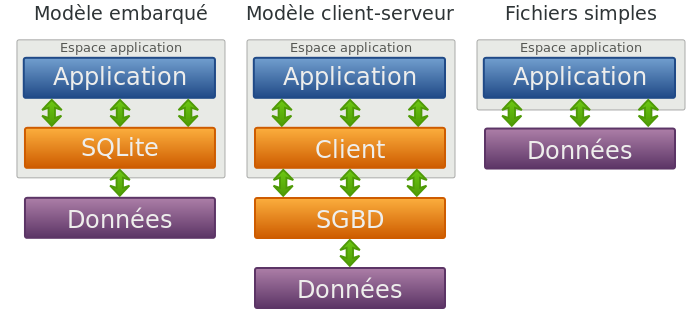
\includegraphics[width=10cm]{ressources/modeles.png}
\captionof{figure}{Modèles d'accès aux données}
\label{modeles}
\end{figure}
\subsection{Un langage}
Les SGBD stockent et optimisent les données de manière efficace mais très complexe. Il n'est pas possible d'y accéder directement. Il faut effectuer des \textbf{requêtes} à l'aide d'un langage adapté.
\begin{aretenir}[]
Le \textbf{SQL (Structured Query Language)} est utilisé dans une écrasante majorité des SGBDR.
\end{aretenir}
Pour la construction d'un site web dynamique, les pages web effectuent des requêtes SQL au serveur MySQL afin de récupérer des données.
\begin{commentprof}
Concurrent: QBE (Query By Example) utilisé dans Microsoft Access	(SGBDR de type "fichier")\\
modèle "fichier simple": traitement de texte; .doc, .odt = xml empaqueté
\end{commentprof}
\begin{figure}[!h]
\centering
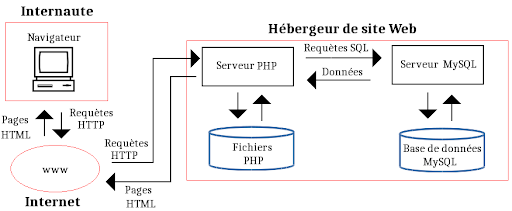
\includegraphics[width=10cm]{ressources/requete-http.png}
\captionof{figure}{Répartition des rôles}
\label{modeles}
\end{figure}
\subsection{Application}
Pour des contraintes d'installation, nous utiliserons dans un premier temps, un modèle SQLite.
\begin{activite}
\begin{enumerate}
\item Télécharger et extraire la version portable de \emph{DB Browser for SQLite} depuis le site officiel \mbox{\url{https://sqlitebrowser.org/dl/}}
\item Télécharger et extraire la base \emph{bd-init.zip} depuis le site \mbox{\url{https://cviroulaud.github.io}}
\item Ouvrir la base avec le browser.
\item Se concentrer d'abord sur l'onglet \emph{Parcourir les données} et observer les tables existantes.
\begin{commentprof}
La table sqlite\_sequence est interne au logiciel.
\end{commentprof}
\end{enumerate}
\end{activite}
\section{Contraintes d'intégrité}
Le modèle relationnel établit des contraintes qui garantissent l'intégrité des données.
\subsection{Contrainte de domaine}
Aux domaines abstraits du modèle relationnel correspondent les types de données du langage SQL.
\begin{center}
\begin{tabular}{|c|c|}
\hline 
\textbf{Nom du type} & \textbf{Description} \\ 
\hline 
SMALLINT & Entier 16 bits signé \\ 
\hline 
INT & Entier 32 bits signé \\ 
\hline 
BIGINT & Entier 64 bit signé \\ 
\hline 
REAL & Flottant 32 bits \\ 
\hline 
CHAR(n) & Chaîne de n caractères exactement \\ 
\hline 
VARCHAR(n) & Chaîne d'au plus n caractères \\ 
\hline 
TEXT & Chaîne de taille quelconque \\ 
\hline 
DATE & Date au format AAAA-MM-JJ \\ 
\hline 
TIME & Heure au format hh:mm:ss \\ 
\hline 
TIMESTAMP & Instant au format AAAA-MM-JJ hh:mm:ss \\ 
\hline 
\end{tabular}
\end{center}
\begin{commentprof}
TINYINT = 1 octet = 0 à 255\\
les flottants sont des valeurs approchées\\
\textbf{DOUBLE PRECISION}: float 64\\
\textbf{DECIMAL}: représente nb à virgules de manière exacte\\
Il existe un \textbf{BOOLEAN} mais inégalement supporté par les SGBD (car pas obligatoire dans les spécifications SQL); pour faire un booléan: CHAR(1)\\
SMALLINT 2 octets = $-2^{15} à 2^{15}-1$; on peut préciser non signé en MySQL (pour id)´
\end{commentprof}
\begin{activite}
\begin{enumerate}
\item Quelle est la valeur maximale que peut prendre un SMALLINT?
\item Quelle sa taille en mémoire?
\item Dans le browser, se rendre dans l'onglet \emph{Structure de la base de données}.
\item Dérouler la table \emph{Auteurs} et repérer les types de chaque attribut.
\end{enumerate}
\end{activite}
Le SGBD Sqlite simplifie les types (INTEGER, REAL, TEXT) en l'adaptant dynamiquement en fonction de la valeur stockée.
\subsection{Contrainte d'entité}
Chaque entité est identifiée de manière unique grâce à la \emph{clé primaire}.
\begin{activite}
\begin{enumerate}
\item Dans le schéma de la table \emph{Auteurs} comment identifie-t-on la clé primaire?
\item Quel est le rôle du mot clé \emph{AUTOINCREMENT}?
\end{enumerate}
\end{activite}
\subsection{Contrainte de référence}
Afin de garantir la cohérence des données lors de modifications, une \emph{clé étrangère} peut être mise en place. C'est une référence à une clé primaire d'une autre relation.
\begin{activite}
\begin{enumerate}
\item Dérouler la table \emph{Bandes\_dessinees}.
\item Rappeler les attributs qui sont des clés étrangères.
\item Glisser la souris sur le schéma de cette table. Quels mots clés sont utilisés pour créer une clé étrangère?
\end{enumerate}
\end{activite}
\subsection{Compléter la base de données}
Afin de pouvoir gérer les emprunts de bandes dessinées, il faut créer les tables \emph{Emprunteurs} et Emprunts.
\begin{activite}
Depuis l'onglet \emph{Exécuter le SQL}, créer ces deux tables, en prenant modèle sur les schémas des relations existantes.
\end{activite}
\begin{aretenir}[Remarque]
Le langage SQL est insensible à la casse. Nous pouvons écrire indifféremment \emph{CREATE} ou \emph{CreaTE}. Il est d'usage d'écrire les instructions SQL en majuscules.
\end{aretenir}
\end{Form}
\end{document}